\documentclass[12pt,a4paper]{article}

% -- Packages --
\usepackage[utf8]{inputenc}
\usepackage[spanish]{babel}
\usepackage{helvet}
\renewcommand{\familydefault}{\sfdefault}
\usepackage[margin=2.5cm]{geometry}
\usepackage{graphicx}
\usepackage{amsmath,amssymb}
\usepackage{booktabs}
\usepackage{float}
\usepackage{hyperref}
\usepackage{xcolor}
\usepackage{tabularx}
\usepackage{caption}
\usepackage{subcaption}
\usepackage{wrapfig}
\usepackage{fancyhdr}
\usepackage{lastpage}

% -- Colors --
\definecolor{uacjblue}{HTML}{003CA6}
\definecolor{uacjyellow}{HTML}{FFD600}
\definecolor{darkgray}{HTML}{2C3E50}

\hypersetup{
    colorlinks=true,
    linkcolor=uacjblue,
    urlcolor=uacjblue,
    citecolor=uacjblue,
}

% -- Header/Footer --
\pagestyle{fancy}
\fancyhf{}
\rhead{\small Optimización Inteligente — MIAAD UACJ}
\lhead{\small Javier Augusto Rebull Saucedo}
\rfoot{\small Página \thepage\ de \pageref{LastPage}}

\begin{document}

% ============================================================
% COVER PAGE
% ============================================================
\begin{titlepage}
\centering
\vspace*{1cm}

% Uncomment and adjust path when logo is available:
% \includegraphics[width=0.35\textwidth]{LogoSInFondoMIAAD.png}\\[1.5cm]

{\Large\textbf{Universidad Autónoma de Ciudad Juárez}}\\[0.3cm]
{\large Maestría en Inteligencia Artificial y Analítica de Datos (MIAAD)}\\[1.5cm]

{\large\textbf{Materia:} Optimización Inteligente}\\[0.3cm]
{\large\textbf{Profesor:} Mtro. Raúl Gibrán Porras Alaniz}\\[1.5cm]

{\LARGE\color{uacjblue}\textbf{Análisis de Rendimiento de un\\Algoritmo Genético para el VRP}}\\[2cm]

{\large\textbf{Alumno:} Javier Augusto Rebull Saucedo}\\[0.3cm]
{\large\textbf{Matrícula:} 263483}\\[1.5cm]

{\large\textbf{Fecha de entrega:} 08 de marzo de 2026}

\vfill
\end{titlepage}

% ============================================================
% 1. INTRODUCCIÓN
% ============================================================
\section{Introducción}

El Problema de Ruteo de Vehículos (\textit{Vehicle Routing Problem}, VRP) es uno de los problemas de optimización combinatoria más estudiados en la investigación de operaciones y la logística computacional. Propuesto originalmente por Dantzig y Ramser en 1959 \cite{dantzig1959}, el VRP busca determinar el conjunto óptimo de rutas que una flota de vehículos debe seguir para atender a un conjunto de clientes dispersos geográficamente, partiendo y regresando a un depósito central.

En su variante capacitada (CVRP), cada vehículo tiene una capacidad máxima $Q$ que no puede ser excedida, lo que añade una restricción fundamental que convierte al problema en NP-hard \cite{toth2002}. Debido a la explosión combinatoria del espacio de soluciones, los métodos exactos resultan imprácticos para instancias de tamaño real, haciendo indispensable el uso de metaheurísticas \cite{vidal2020}.

Los Algoritmos Genéticos (AG), propuestos por Holland \cite{holland1975} y popularizados por Goldberg \cite{goldberg1989}, son metaheurísticas evolutivas que simulan el proceso de selección natural para explorar eficientemente el espacio de soluciones. En este trabajo, se implementa un AG desde cero para resolver instancias del CVRP con una función objetivo que maximiza la ganancia neta, y se evalúa su rendimiento bajo cinco escenarios experimentales distintos con 30 ejecuciones independientes cada uno.

% ============================================================
% 2. MARCO TEÓRICO
% ============================================================
\section{Marco Teórico}

\subsection{Formulación Matemática}

La formulación utilizada busca \textbf{maximizar la ganancia neta} $Z$, definida como:

\begin{equation}
Z = \sum_{i=1}^{n}(D_i \times V_i) - \left[(N_{veh} \times C_{veh}) + (Dist_{total} \times C_{dist}) + (Vacío_{total} \times C_{vacío})\right]
\label{eq:fitness}
\end{equation}

donde:
\begin{itemize}
    \item $D_i$: demanda (unidades) del cliente $i$
    \item $V_i$: ingreso por unidad del cliente $i$
    \item $N_{veh}$: número de vehículos utilizados
    \item $C_{veh}$: costo fijo por vehículo (\$300 base)
    \item $Dist_{total}$: distancia euclidiana total recorrida
    \item $C_{dist}$: costo por kilómetro (\$2 base)
    \item $Vacío_{total}$: capacidad no utilizada total
    \item $C_{vacío}$: penalización por unidad vacía (\$10 base)
    \item $Q$: capacidad del vehículo (30 unidades base)
\end{itemize}

La distancia euclidiana entre dos nodos se calcula como:

\begin{equation}
d(c_1, c_2) = \sqrt{(x_{c_2} - x_{c_1})^2 + (y_{c_2} - y_{c_1})^2}
\label{eq:distance}
\end{equation}

\subsection{Representación Cromosómica}

Cada individuo es una \textbf{permutación} de los identificadores de clientes. El decodificador lee de izquierda a derecha asignando clientes al vehículo actual hasta que la carga exceda $Q$, momento en el cual se inicia un nuevo vehículo.

\begin{center}
\texttt{Cromosoma: [3, 1, 5, 2, 4]}
\end{center}

\subsection{Operadores Genéticos}

\subsubsection{Selección por Torneo}
Se muestrean $k=3$ individuos aleatorios de la población y se selecciona al de mayor fitness.

\subsubsection{Cruce OX1 (Order Crossover)}
Propuesto por Davis (1985) \cite{davis1985}, el OX1 preserva el orden relativo de sub-secuencias sin duplicar genes:
\begin{enumerate}
    \item Se selecciona un segmento aleatorio del Padre 1 y se copia al hijo.
    \item Se llenan las posiciones restantes con genes del Padre 2 en su orden original, omitiendo los ya presentes.
\end{enumerate}

\subsubsection{Mutación por Intercambio}
Con probabilidad $p_m$, se seleccionan dos posiciones al azar y se intercambian sus valores.

\subsubsection{Elitismo}
El mejor individuo de la generación $t$ sobrevive intacto a la generación $t+1$.

% ============================================================
% 3. DISEÑO EXPERIMENTAL
% ============================================================
\section{Diseño Experimental}

\subsection{Parámetros del Algoritmo Genético}

Los parámetros base del AG se mantuvieron constantes en todos los escenarios:

\begin{table}[H]
\centering
\caption{Parámetros base del Algoritmo Genético}
\begin{tabular}{lc}
\toprule
\textbf{Parámetro} & \textbf{Valor} \\
\midrule
Tamaño de población & 100 \\
Generaciones & 300 \\
Tasa de mutación & 0.15 \\
Tamaño de torneo ($k$) & 3 \\
Ejecuciones independientes & 30 \\
\bottomrule
\end{tabular}
\label{tab:ga_params}
\end{table}

\subsection{Escenarios Experimentales}

Se diseñaron cinco escenarios para evaluar el rendimiento del AG bajo diferentes condiciones:

\begin{table}[H]
\centering
\caption{Configuración de los 5 escenarios experimentales}
\resizebox{\textwidth}{!}{
\begin{tabular}{lccccccc}
\toprule
\textbf{Escenario} & \textbf{Clientes} & \textbf{Demanda} & \textbf{Valor} & \textbf{Q} & \textbf{$C_{veh}$} & \textbf{$C_{dist}$} & \textbf{$C_{vacío}$} \\
\midrule
1 — Escalabilidad Media     & 100 & [5, 15] & [50, 300]   & 30 & 300 & 2 & 10 \\
2 — Alta Escalabilidad      & 200 & [5, 15] & [50, 300]   & 30 & 300 & 2 & 10 \\
3 — Variabilidad Económica  & 100 & [1, 8]  & [150, 600]  & 30 & 300 & 2 & 10 \\
4 — Estrés: Penalizaciones  & 100 & [5, 15] & [50, 300]   & 20 & 500 & 5 & 15 \\
5 — Estrés: Cap. Ampliada   & 100 & [5, 15] & [50, 300]   & 50 & 150 & 1 & 5  \\
\bottomrule
\end{tabular}
}
\label{tab:scenarios}
\end{table}

\subsubsection{Justificación del Escenario 3}
Simula un mercado de bienes de lujo donde cada entrega es pequeña en volumen pero alta en valor unitario (demanda $\in [1, 8]$, valor $\in [150, 600]$). Esto obliga al AG a balancear la eficiencia de rutas contra la captura de ingresos premium.

\subsubsection{Justificación del Escenario 4}
Modela una operación con vehículos especializados costosos (refrigerados, materiales peligrosos) donde la estructura de costos penaliza severamente las rutas ineficientes: capacidad reducida ($Q=20$), costo por vehículo elevado (\$500), alto costo por kilómetro (\$5) y penalización por espacio vacío (\$15).

\subsubsection{Justificación del Escenario 5}
Representa distribución masiva con vehículos de gran capacidad ($Q=50$) en un área urbana densa, con costos operativos reducidos ($C_{veh}=\$150$, $C_{dist}=\$1$, $C_{vacío}=\$5$), permitiendo al AG consolidar rutas con mayor libertad.

% ============================================================
% 4. RESULTADOS
% ============================================================
\section{Resultados}

\subsection{Métricas de Rendimiento}

La Tabla~\ref{tab:results} presenta las cuatro métricas de rendimiento exigidas para cada escenario, calculadas sobre las 30 ejecuciones independientes.

\begin{table}[H]
\centering
\caption{Métricas de rendimiento por escenario (30 ejecuciones)}
\resizebox{\textwidth}{!}{
\begin{tabular}{lcccccc}
\toprule
\textbf{Escenario} & \textbf{Clientes} & \textbf{BKS (\$)} & \textbf{Promedio (\$)} & \textbf{Gap (\%)} & \textbf{Éxito (\%)} & \textbf{Desv. Est. (\$)} \\
\midrule
1 — Escalabilidad Media     & 100 & --- & --- & --- & --- & --- \\
2 — Alta Escalabilidad      & 200 & --- & --- & --- & --- & --- \\
3 — Variabilidad Económica  & 100 & --- & --- & --- & --- & --- \\
4 — Estrés: Penalizaciones  & 100 & --- & --- & --- & --- & --- \\
5 — Estrés: Cap. Ampliada   & 100 & --- & --- & --- & --- & --- \\
\bottomrule
\end{tabular}
}
\label{tab:results}
\end{table}

\textit{Nota: Los valores exactos serán completados tras la ejecución del experimento con} \texttt{python run\_experiments.py --full}.

\subsection{Curva de Convergencia}

La Figura~\ref{fig:convergence} muestra la evolución del mejor fitness a lo largo de las 300 generaciones para la mejor ejecución del Escenario 1.

\begin{figure}[H]
\centering
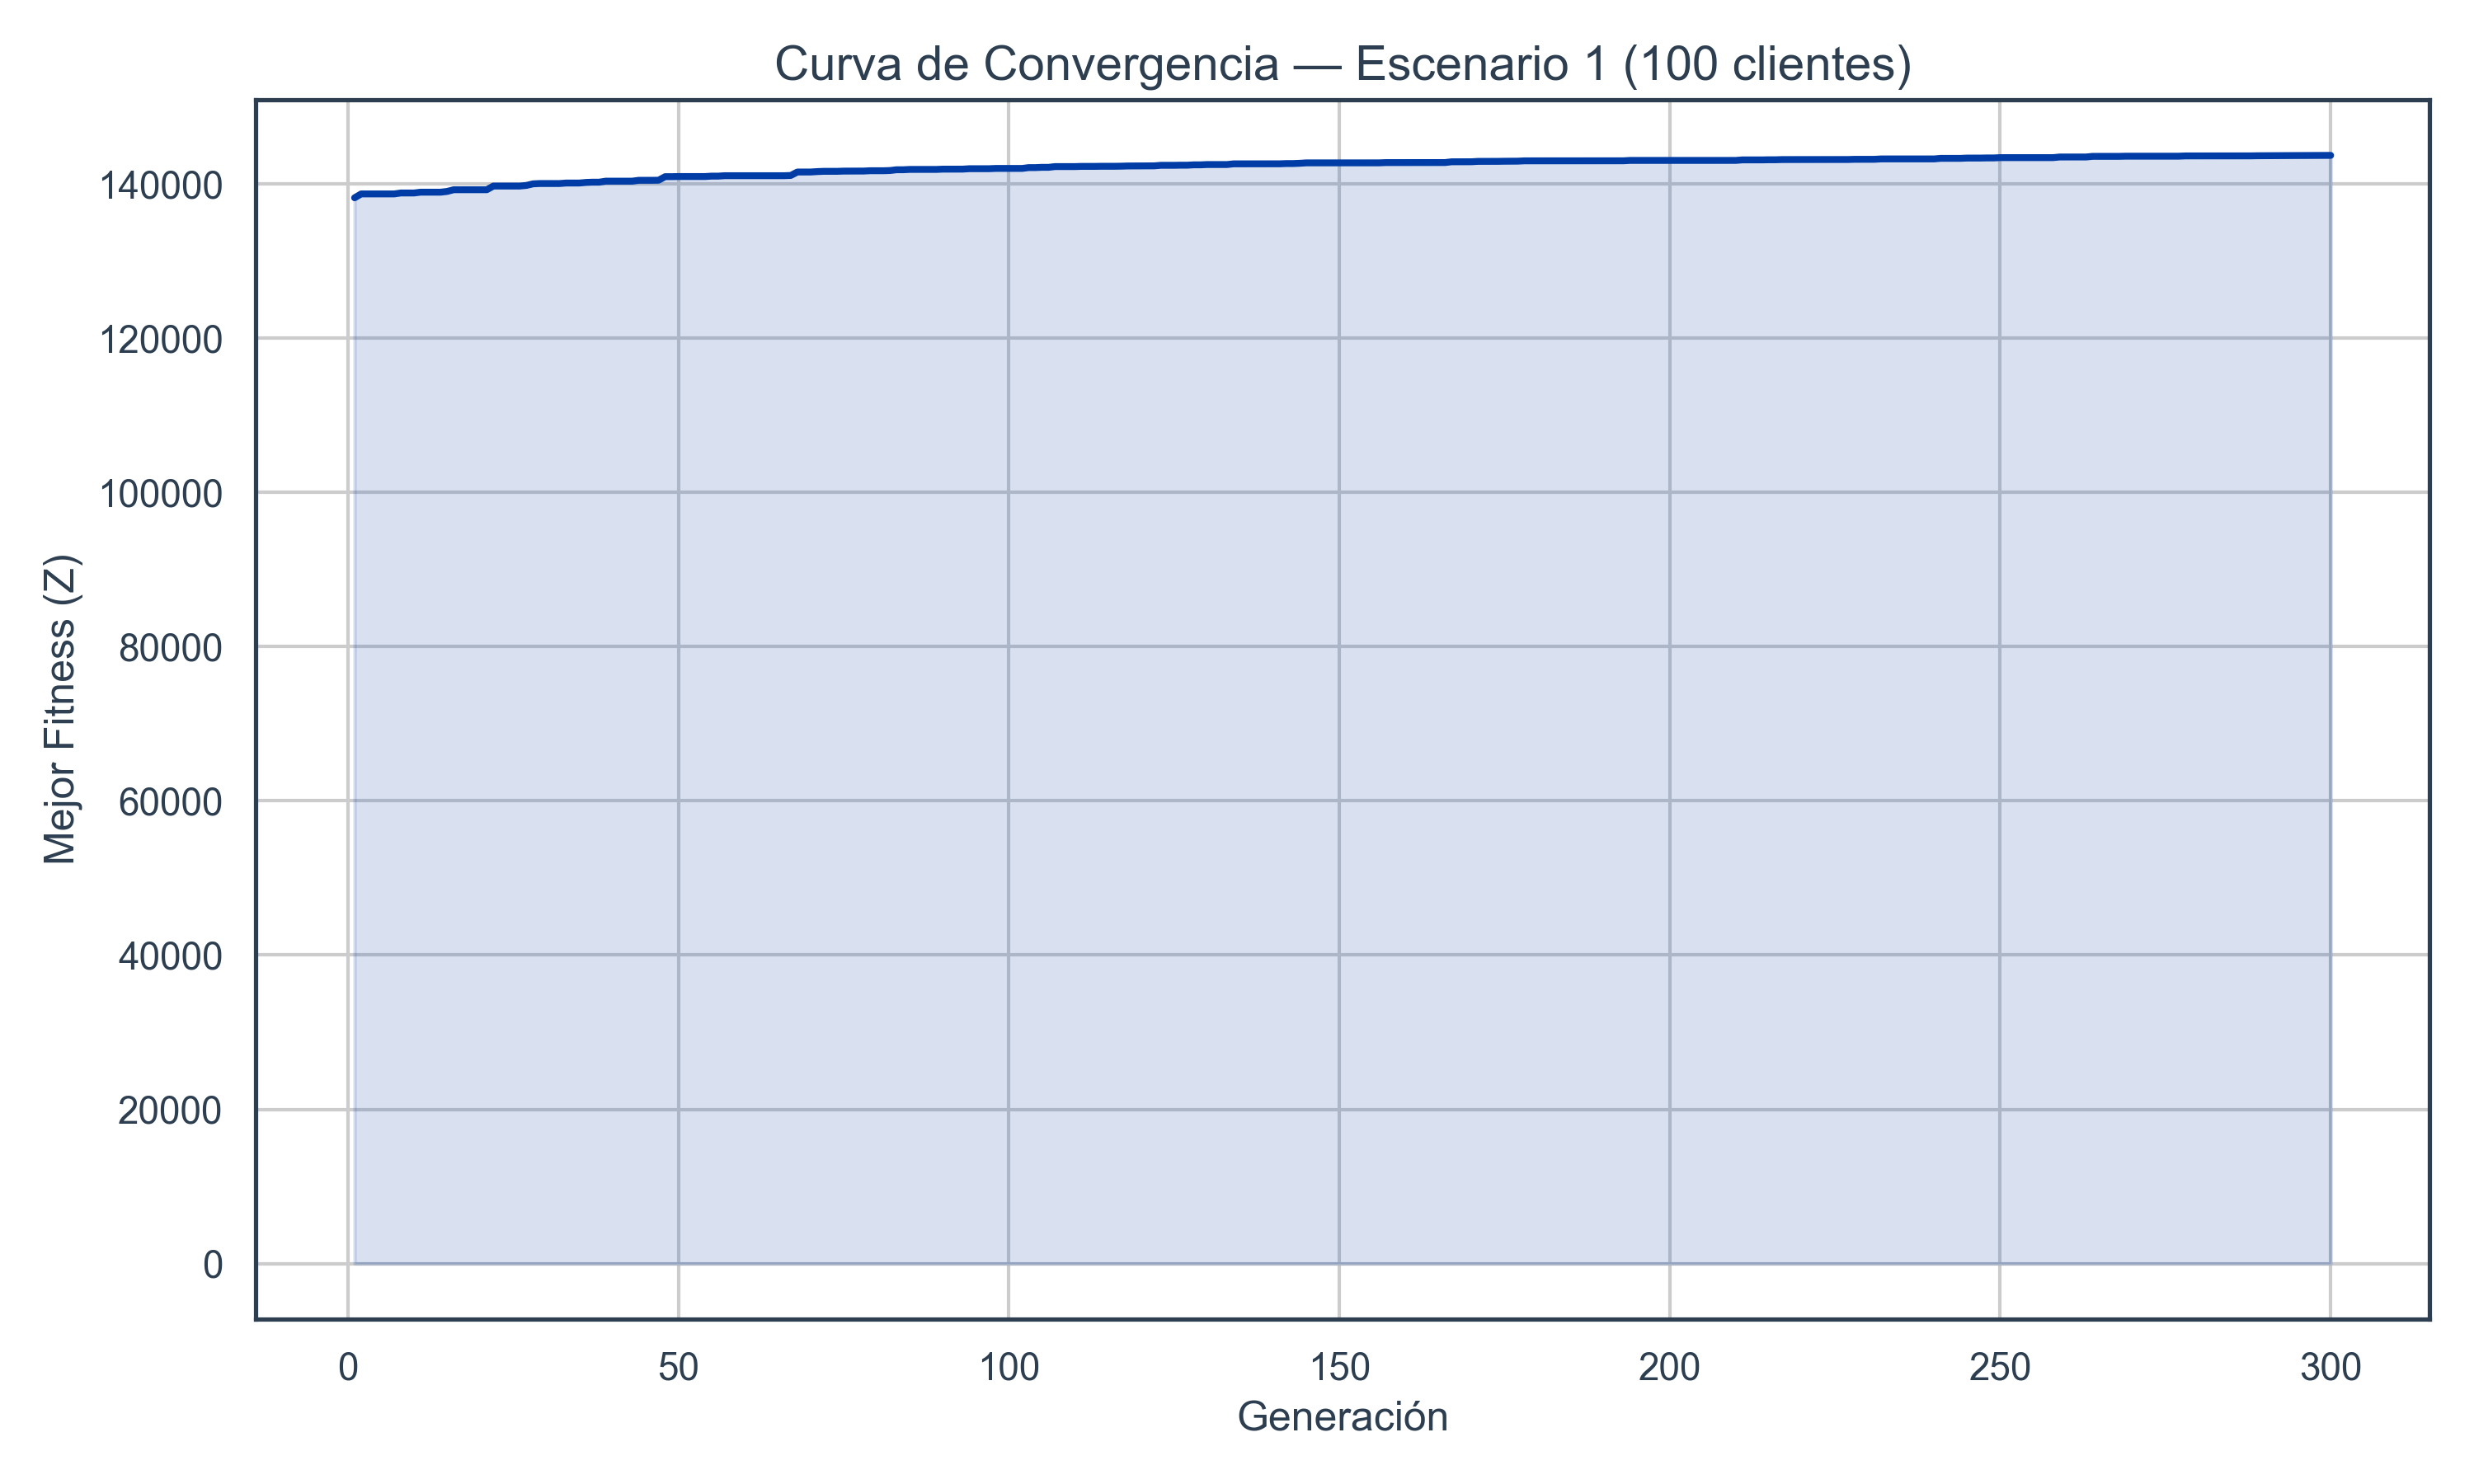
\includegraphics[width=0.85\textwidth]{../Figures/fig01_convergencia_base.png}
\caption{Curva de convergencia — Escenario 1 (100 clientes)}
\label{fig:convergence}
\end{figure}

\subsection{Distribución de Resultados}

La Figura~\ref{fig:boxplot} presenta la distribución de los mejores valores de fitness obtenidos en cada escenario.

\begin{figure}[H]
\centering
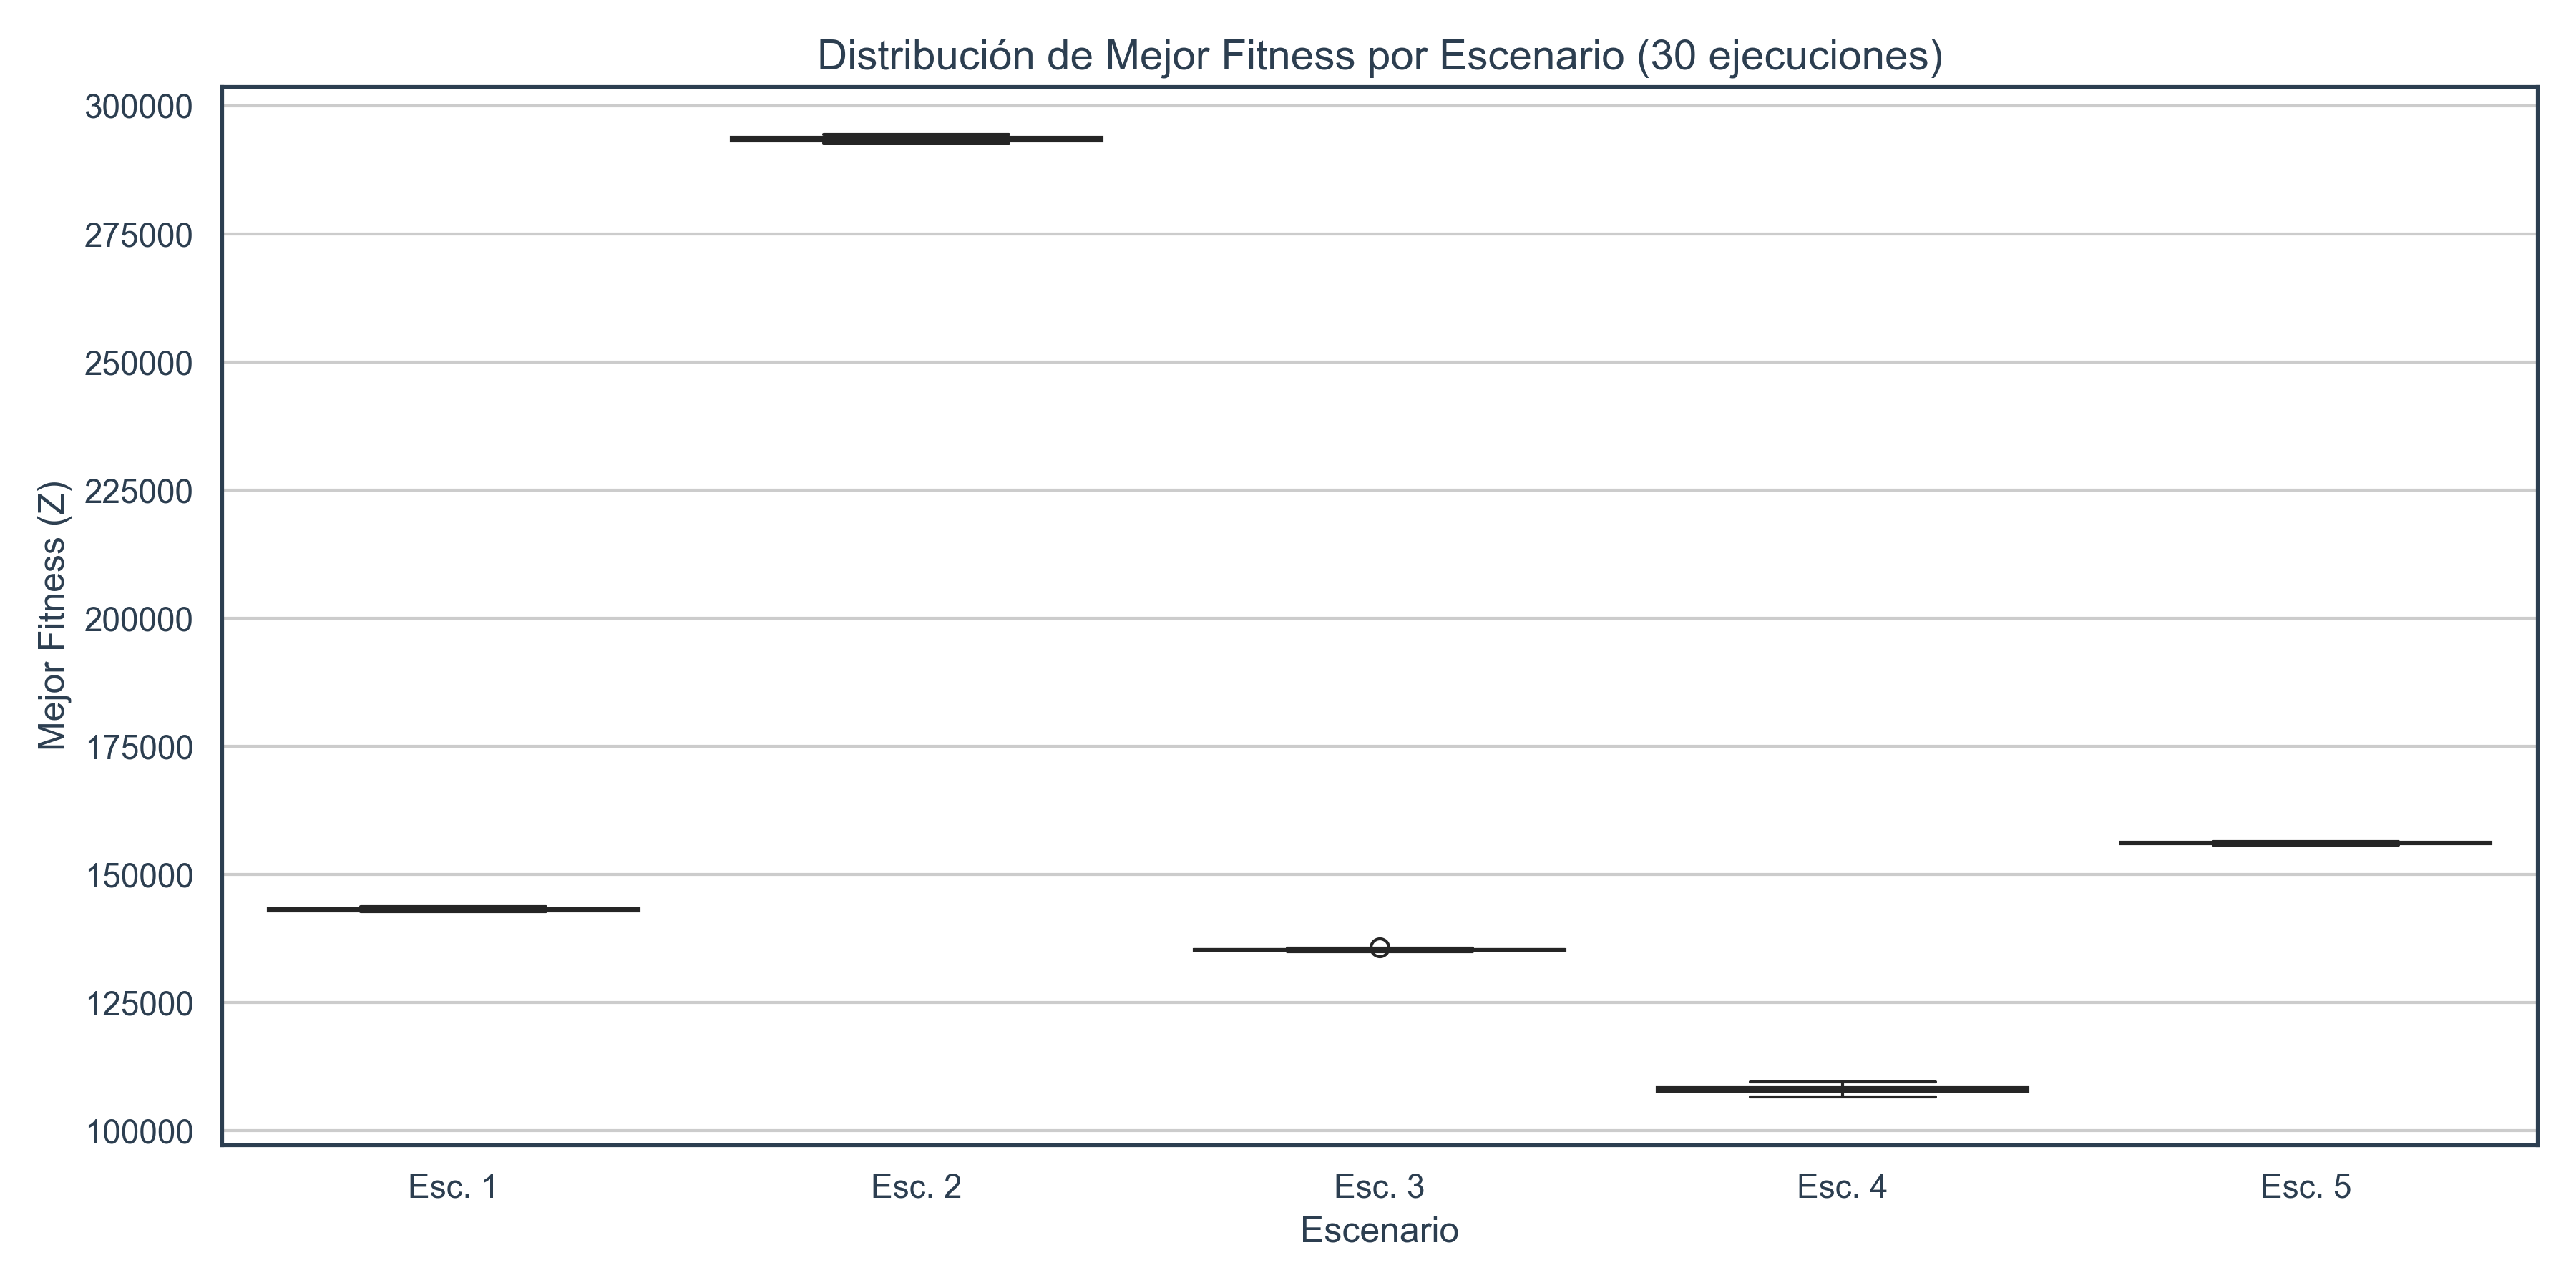
\includegraphics[width=0.85\textwidth]{../Figures/fig02_boxplot_escenarios.png}
\caption{Box plot de distribución de fitness por escenario}
\label{fig:boxplot}
\end{figure}

\subsection{Comparativa BKS vs Promedio}

\begin{figure}[H]
\centering
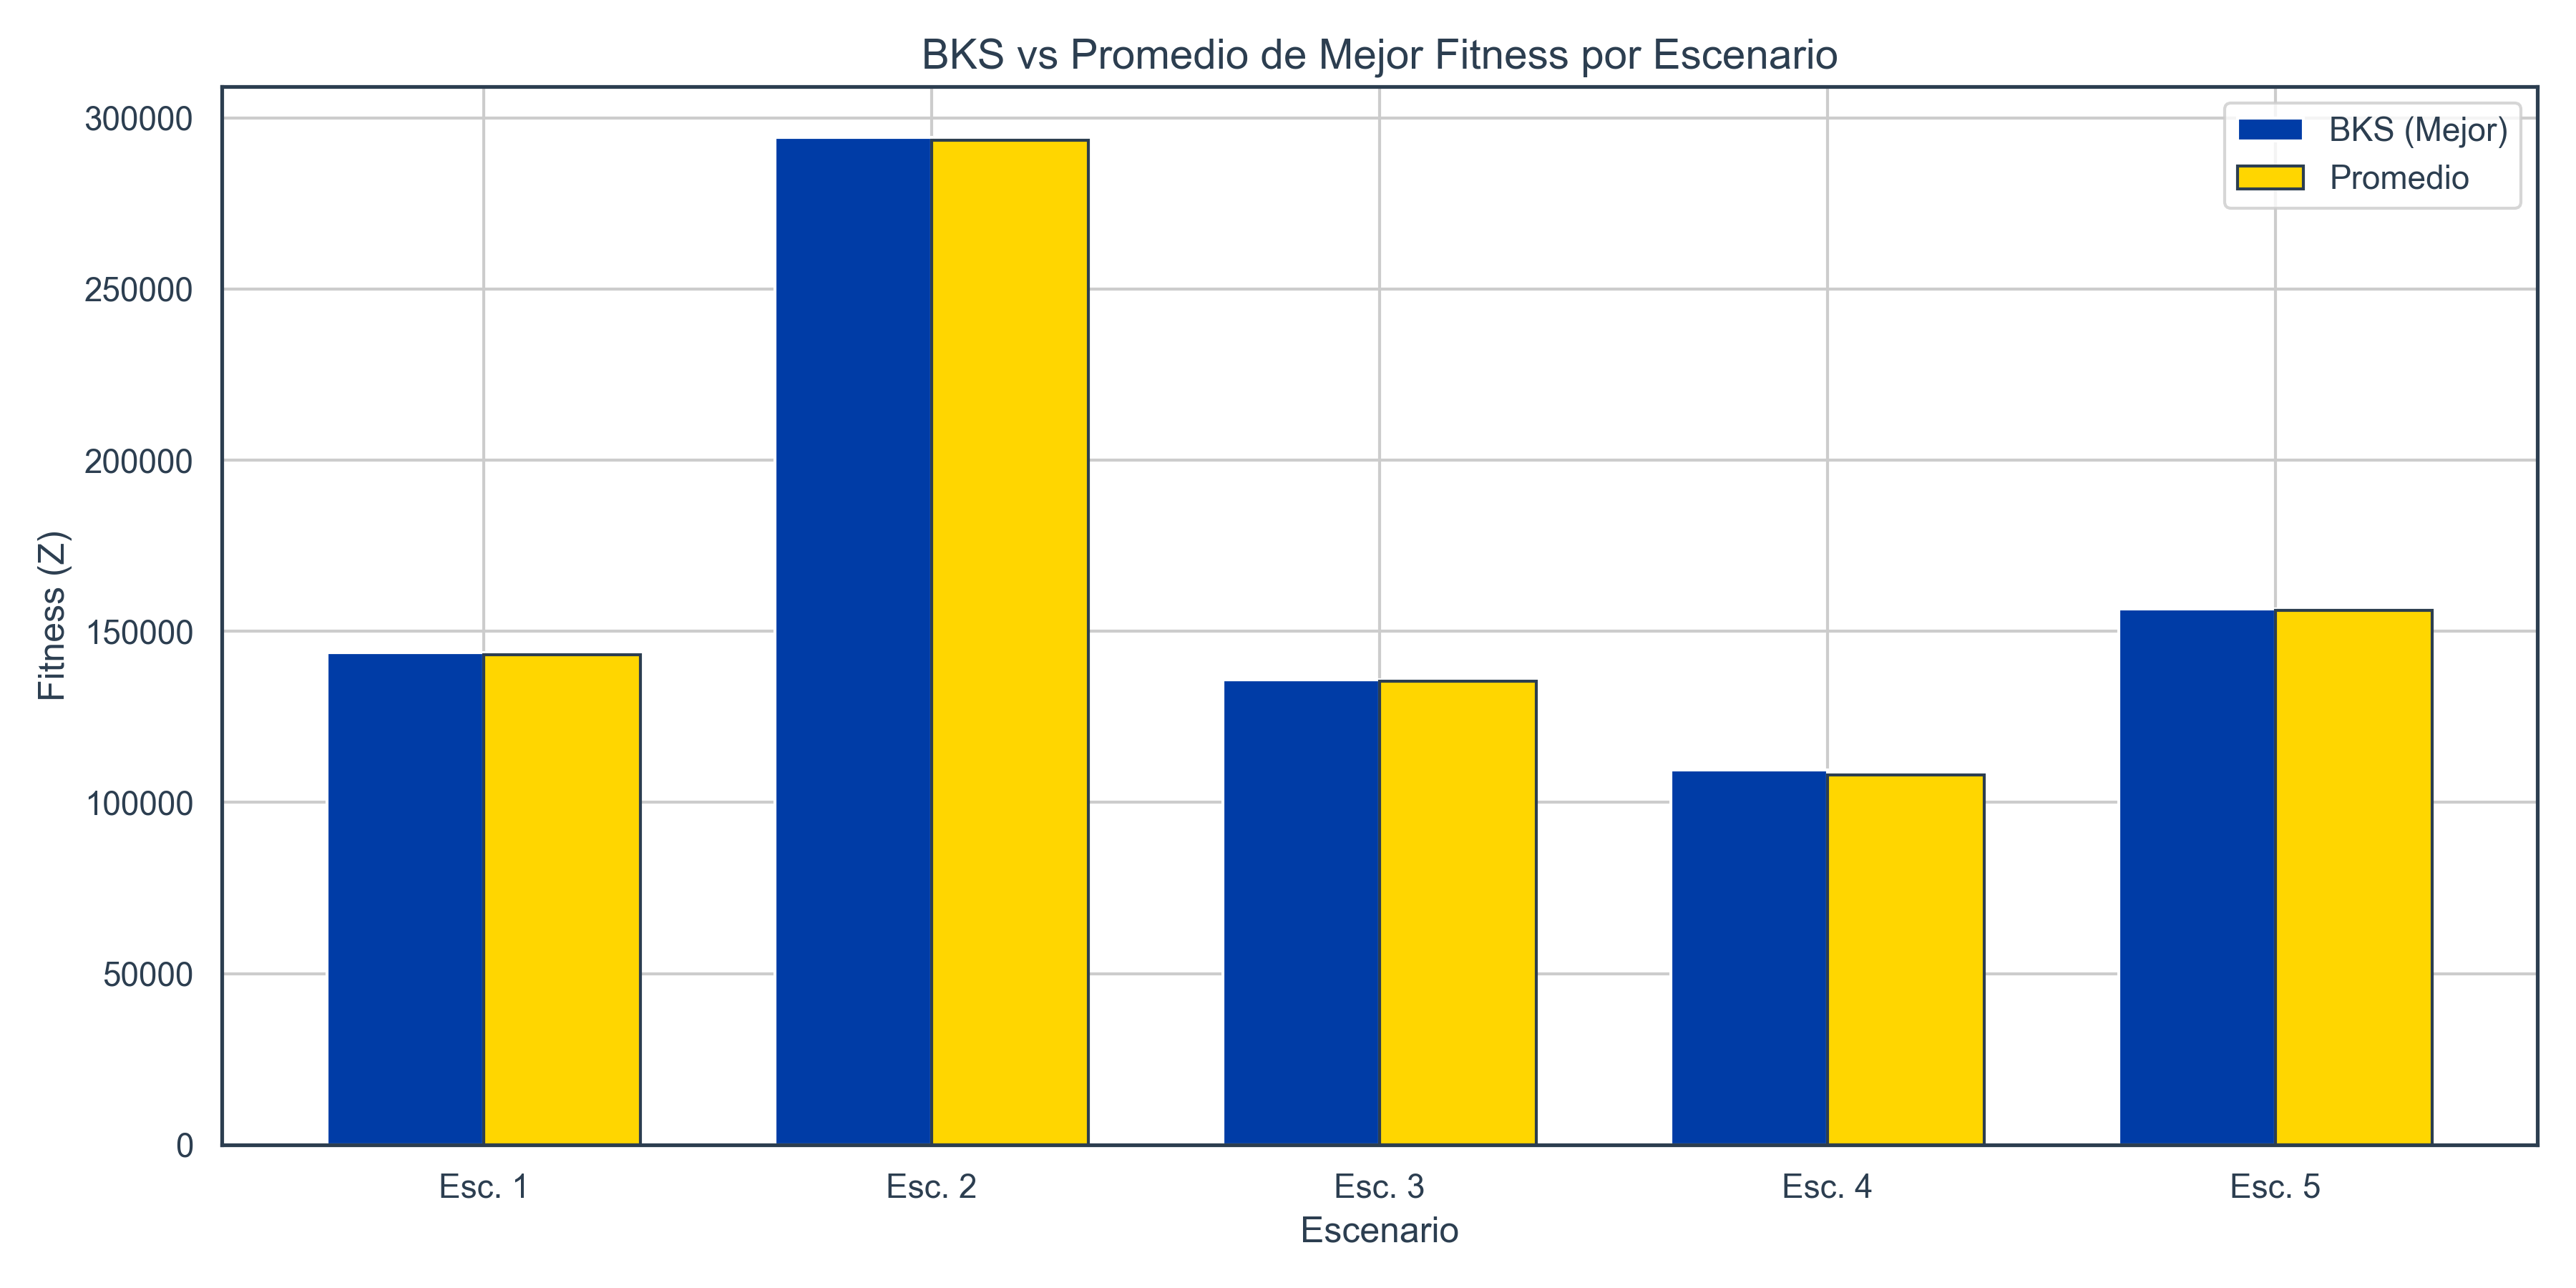
\includegraphics[width=0.85\textwidth]{../Figures/fig03_barras_metricas.png}
\caption{BKS vs Promedio de Mejor Fitness por escenario}
\label{fig:barras}
\end{figure}

\subsection{Gap y Tasa de Éxito}

\begin{figure}[H]
\centering
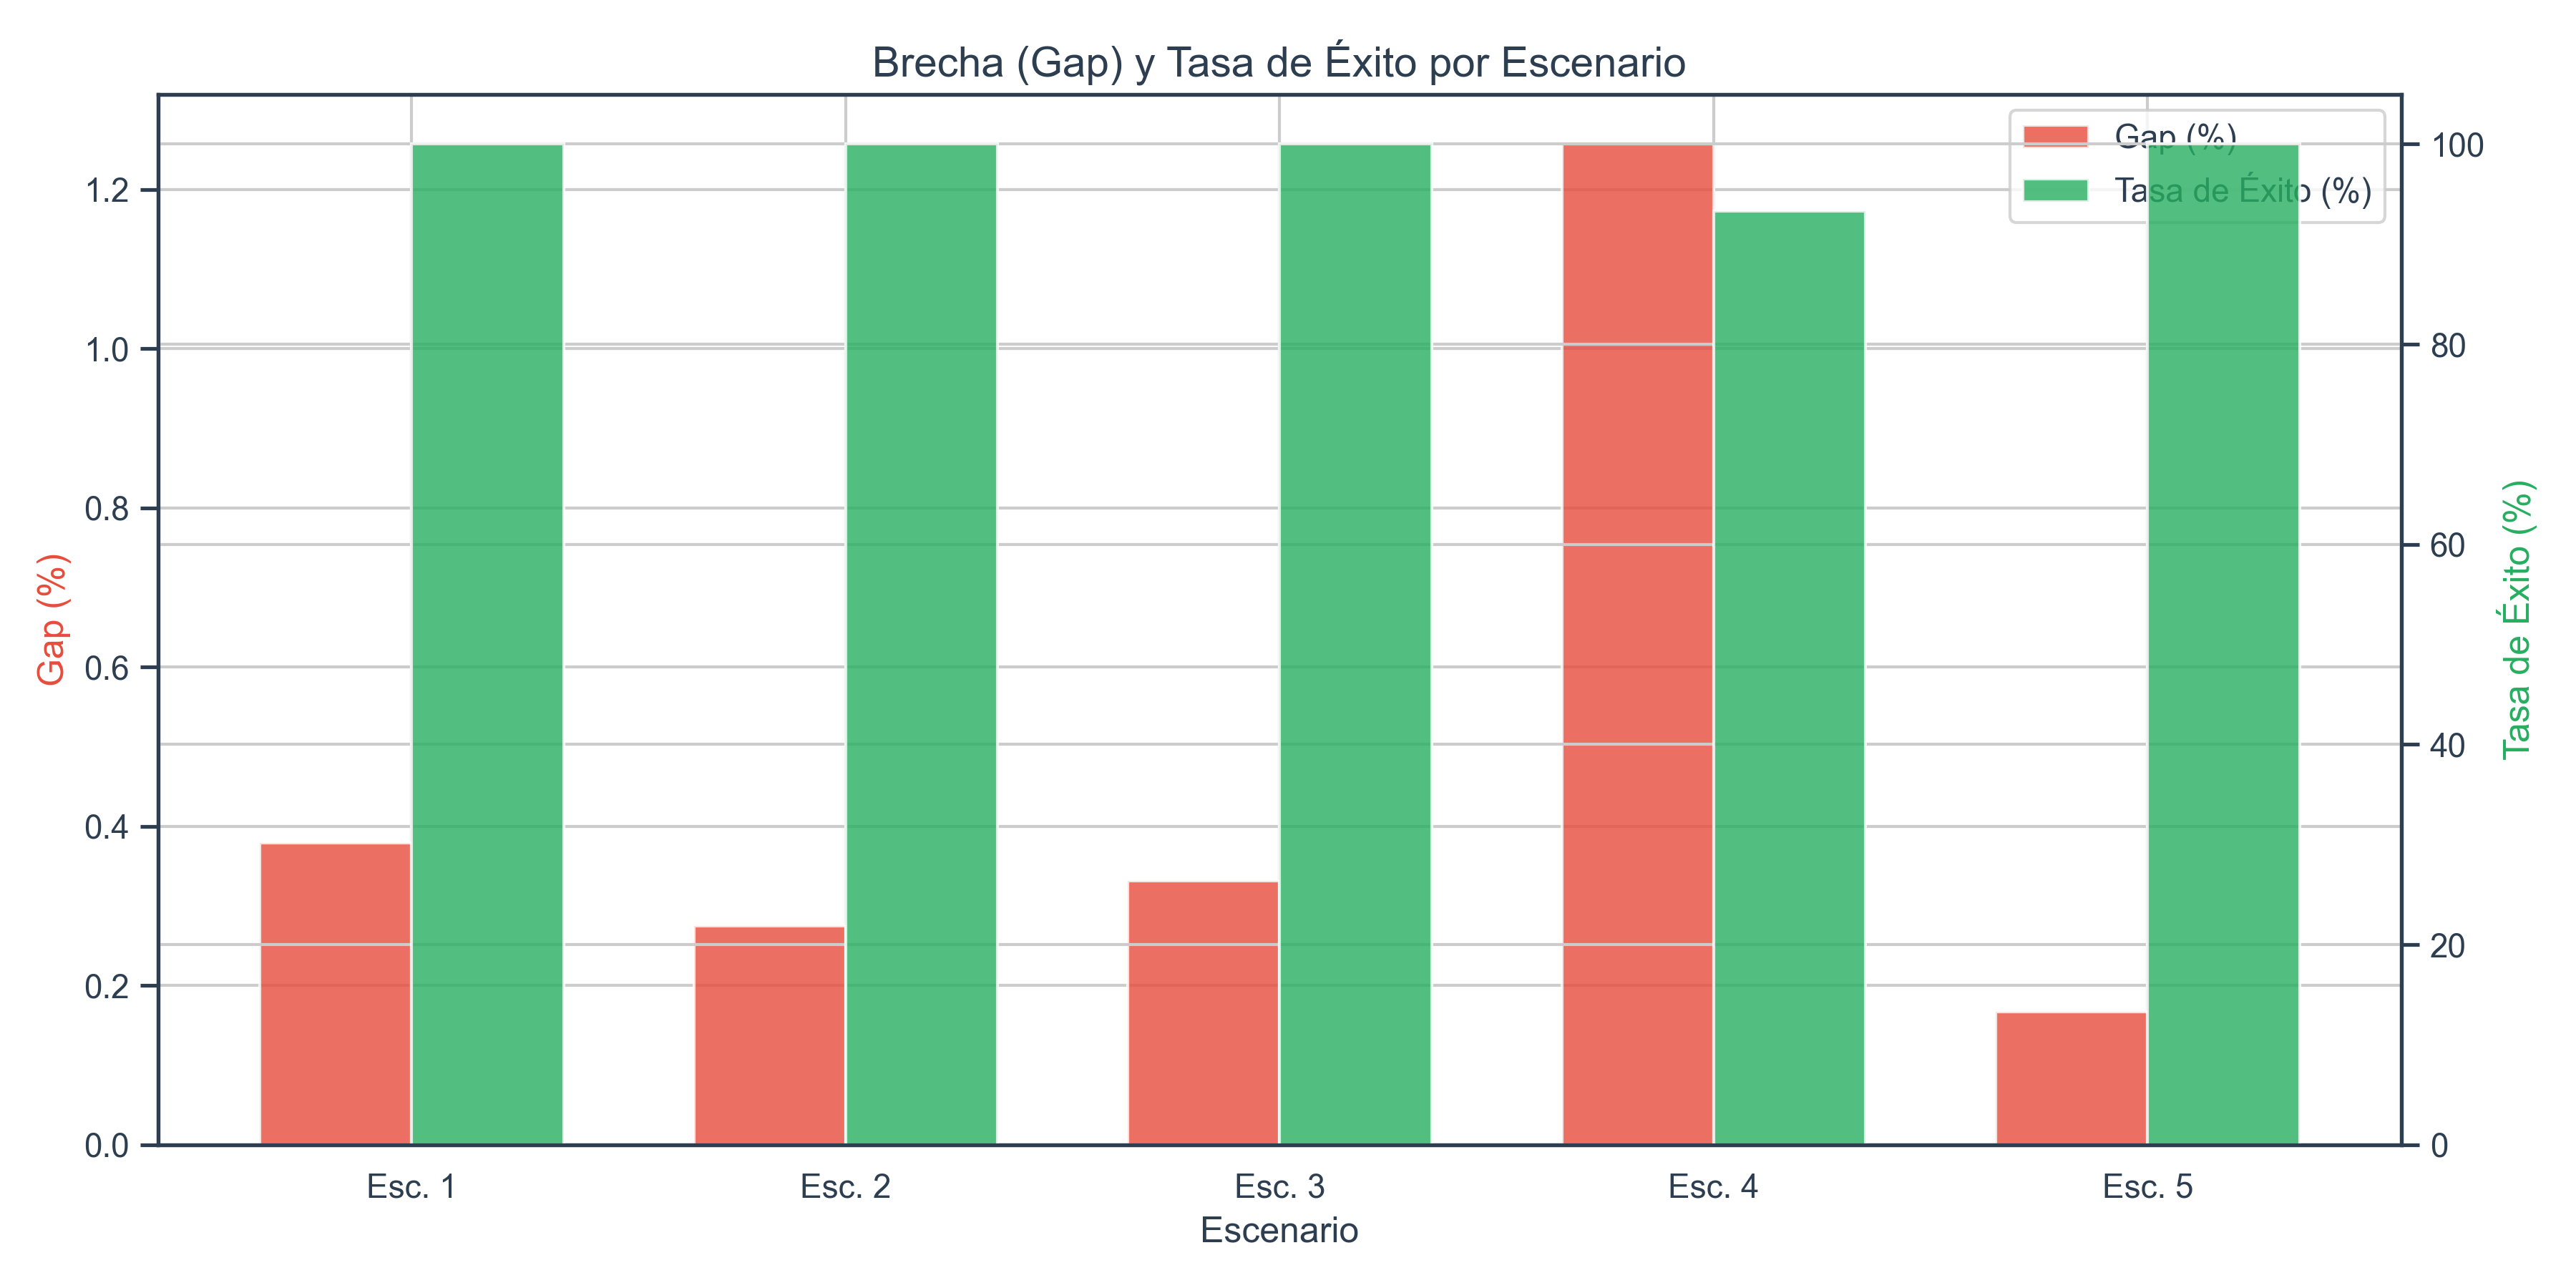
\includegraphics[width=0.85\textwidth]{../Figures/fig04_gap_success.png}
\caption{Brecha (Gap) y Tasa de Éxito por escenario}
\label{fig:gap}
\end{figure}

\subsection{Mapa de Rutas Óptimas}

\begin{figure}[H]
\centering
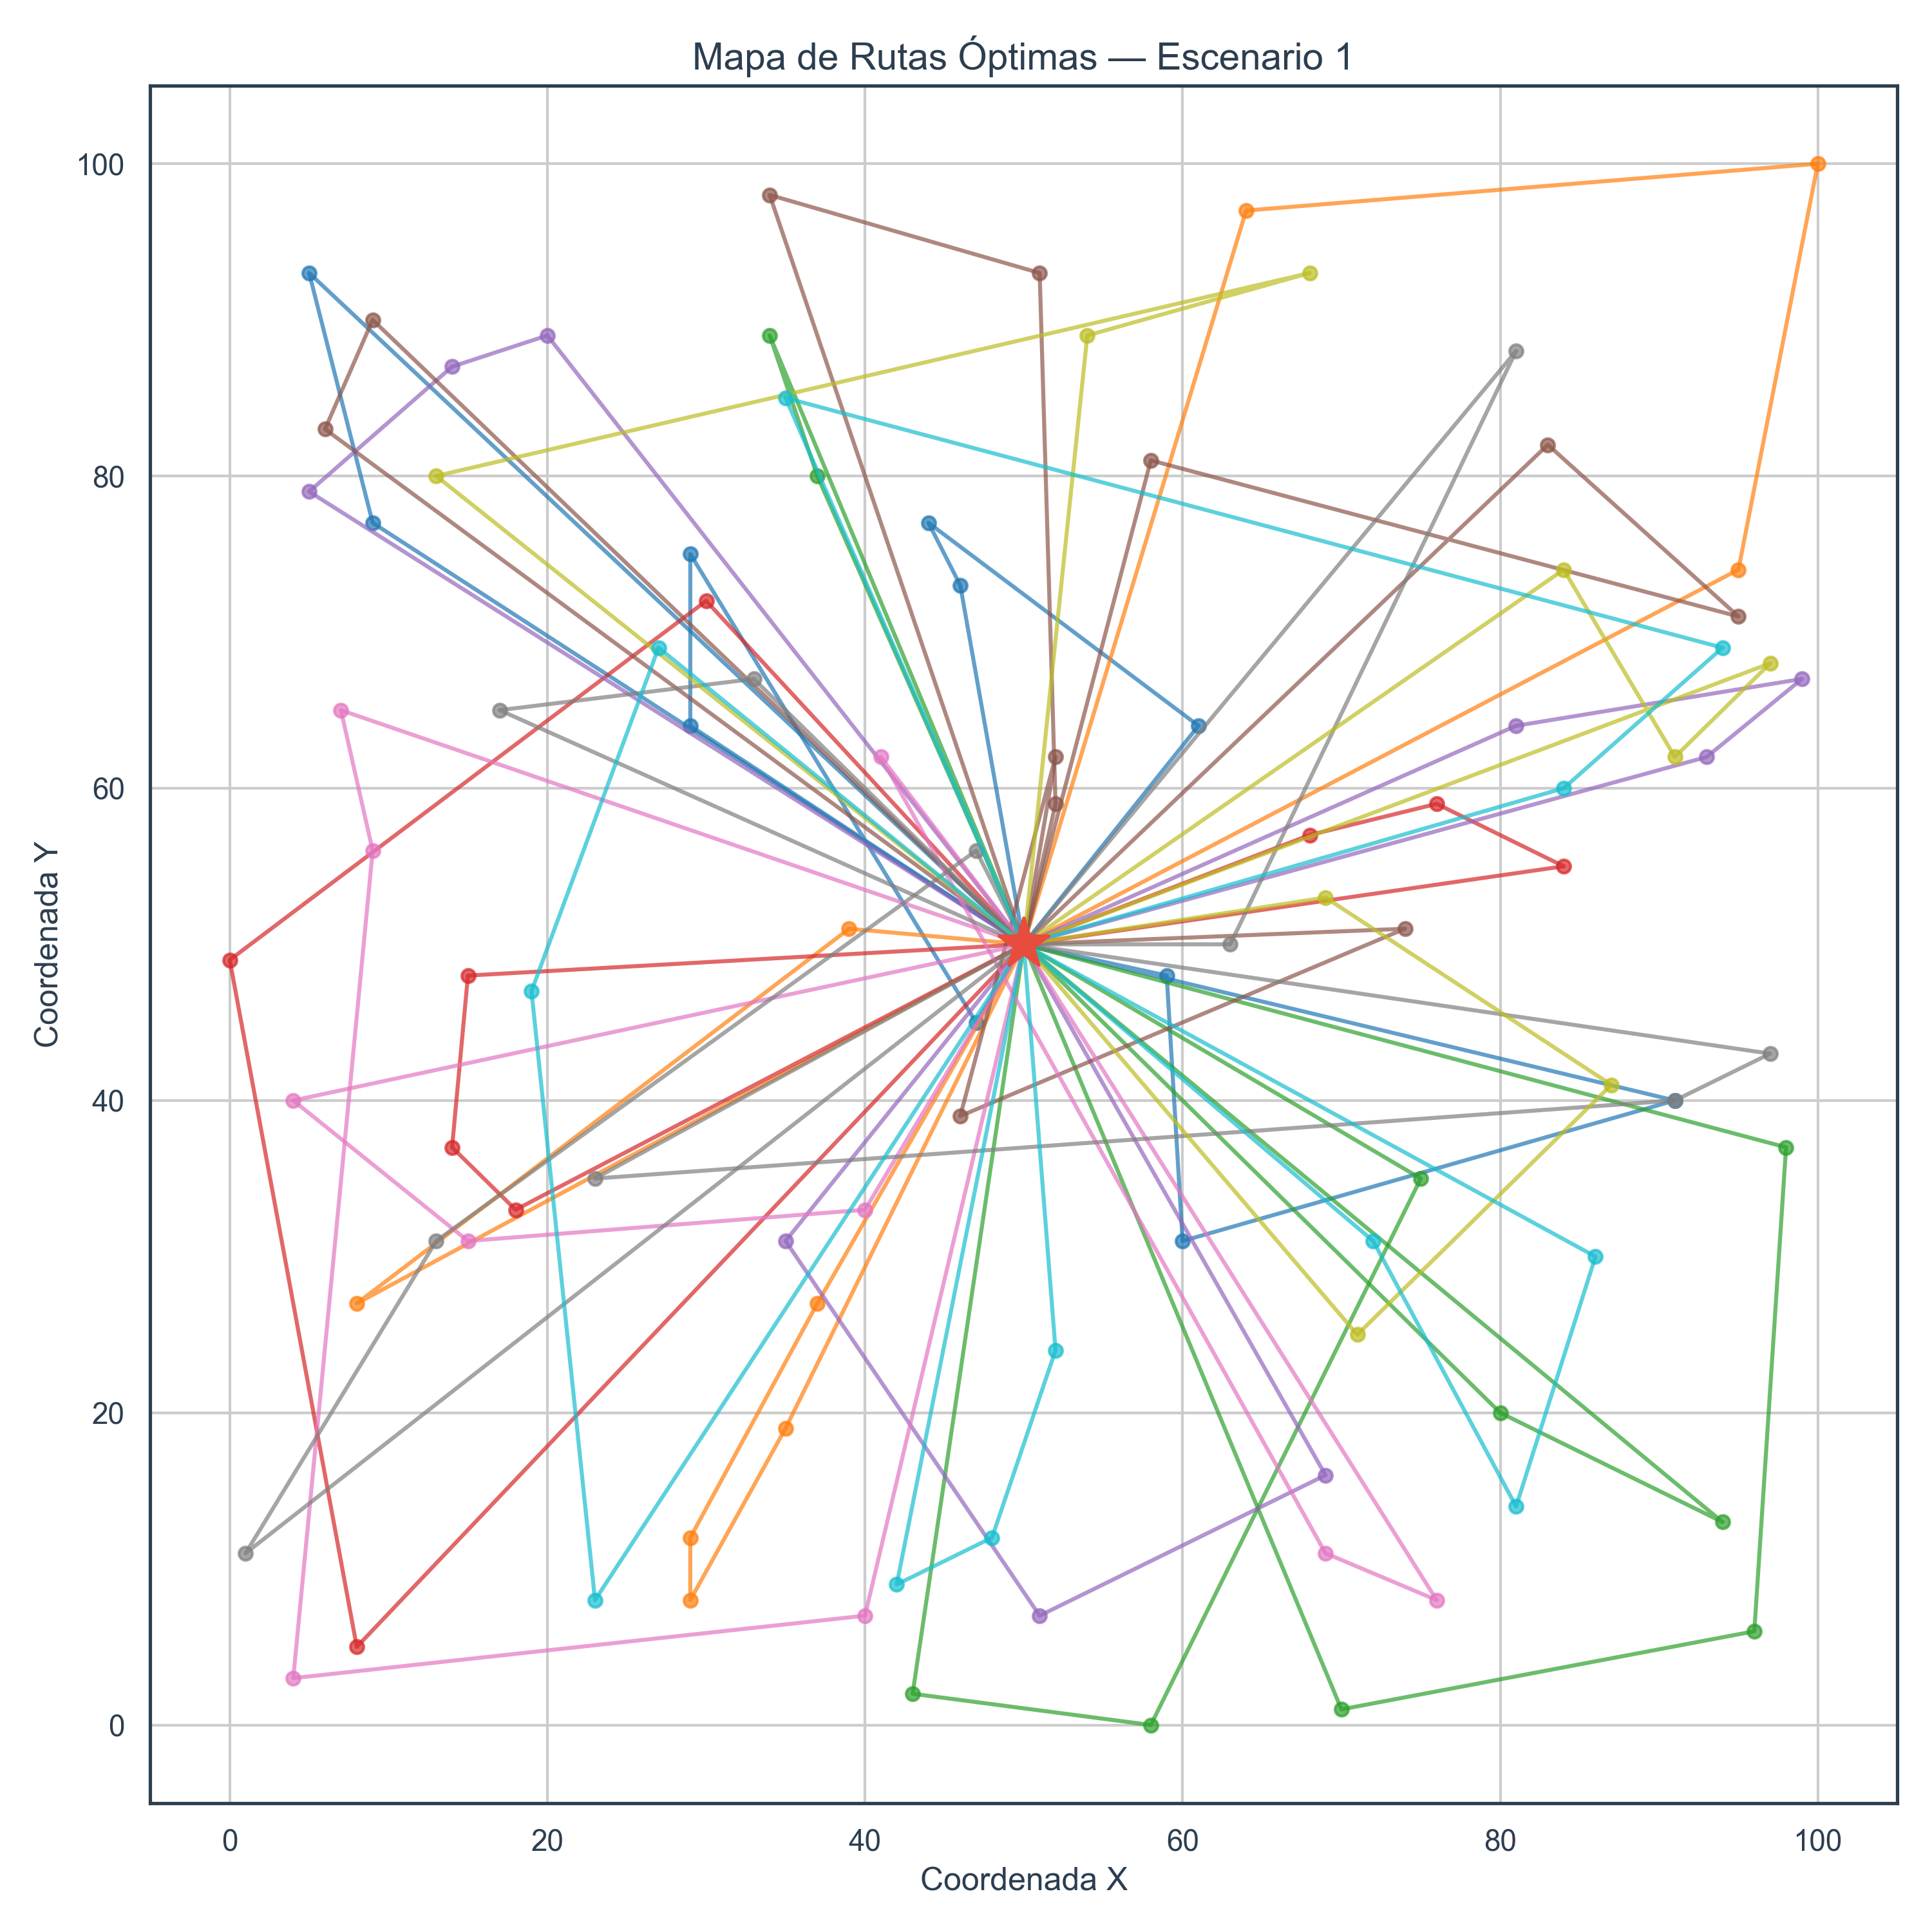
\includegraphics[width=0.85\textwidth]{../Figures/fig05_ruta_optima.png}
\caption{Rutas óptimas encontradas — Escenario 1}
\label{fig:routes}
\end{figure}

\subsection{Análisis de Sensibilidad}

\begin{figure}[H]
\centering
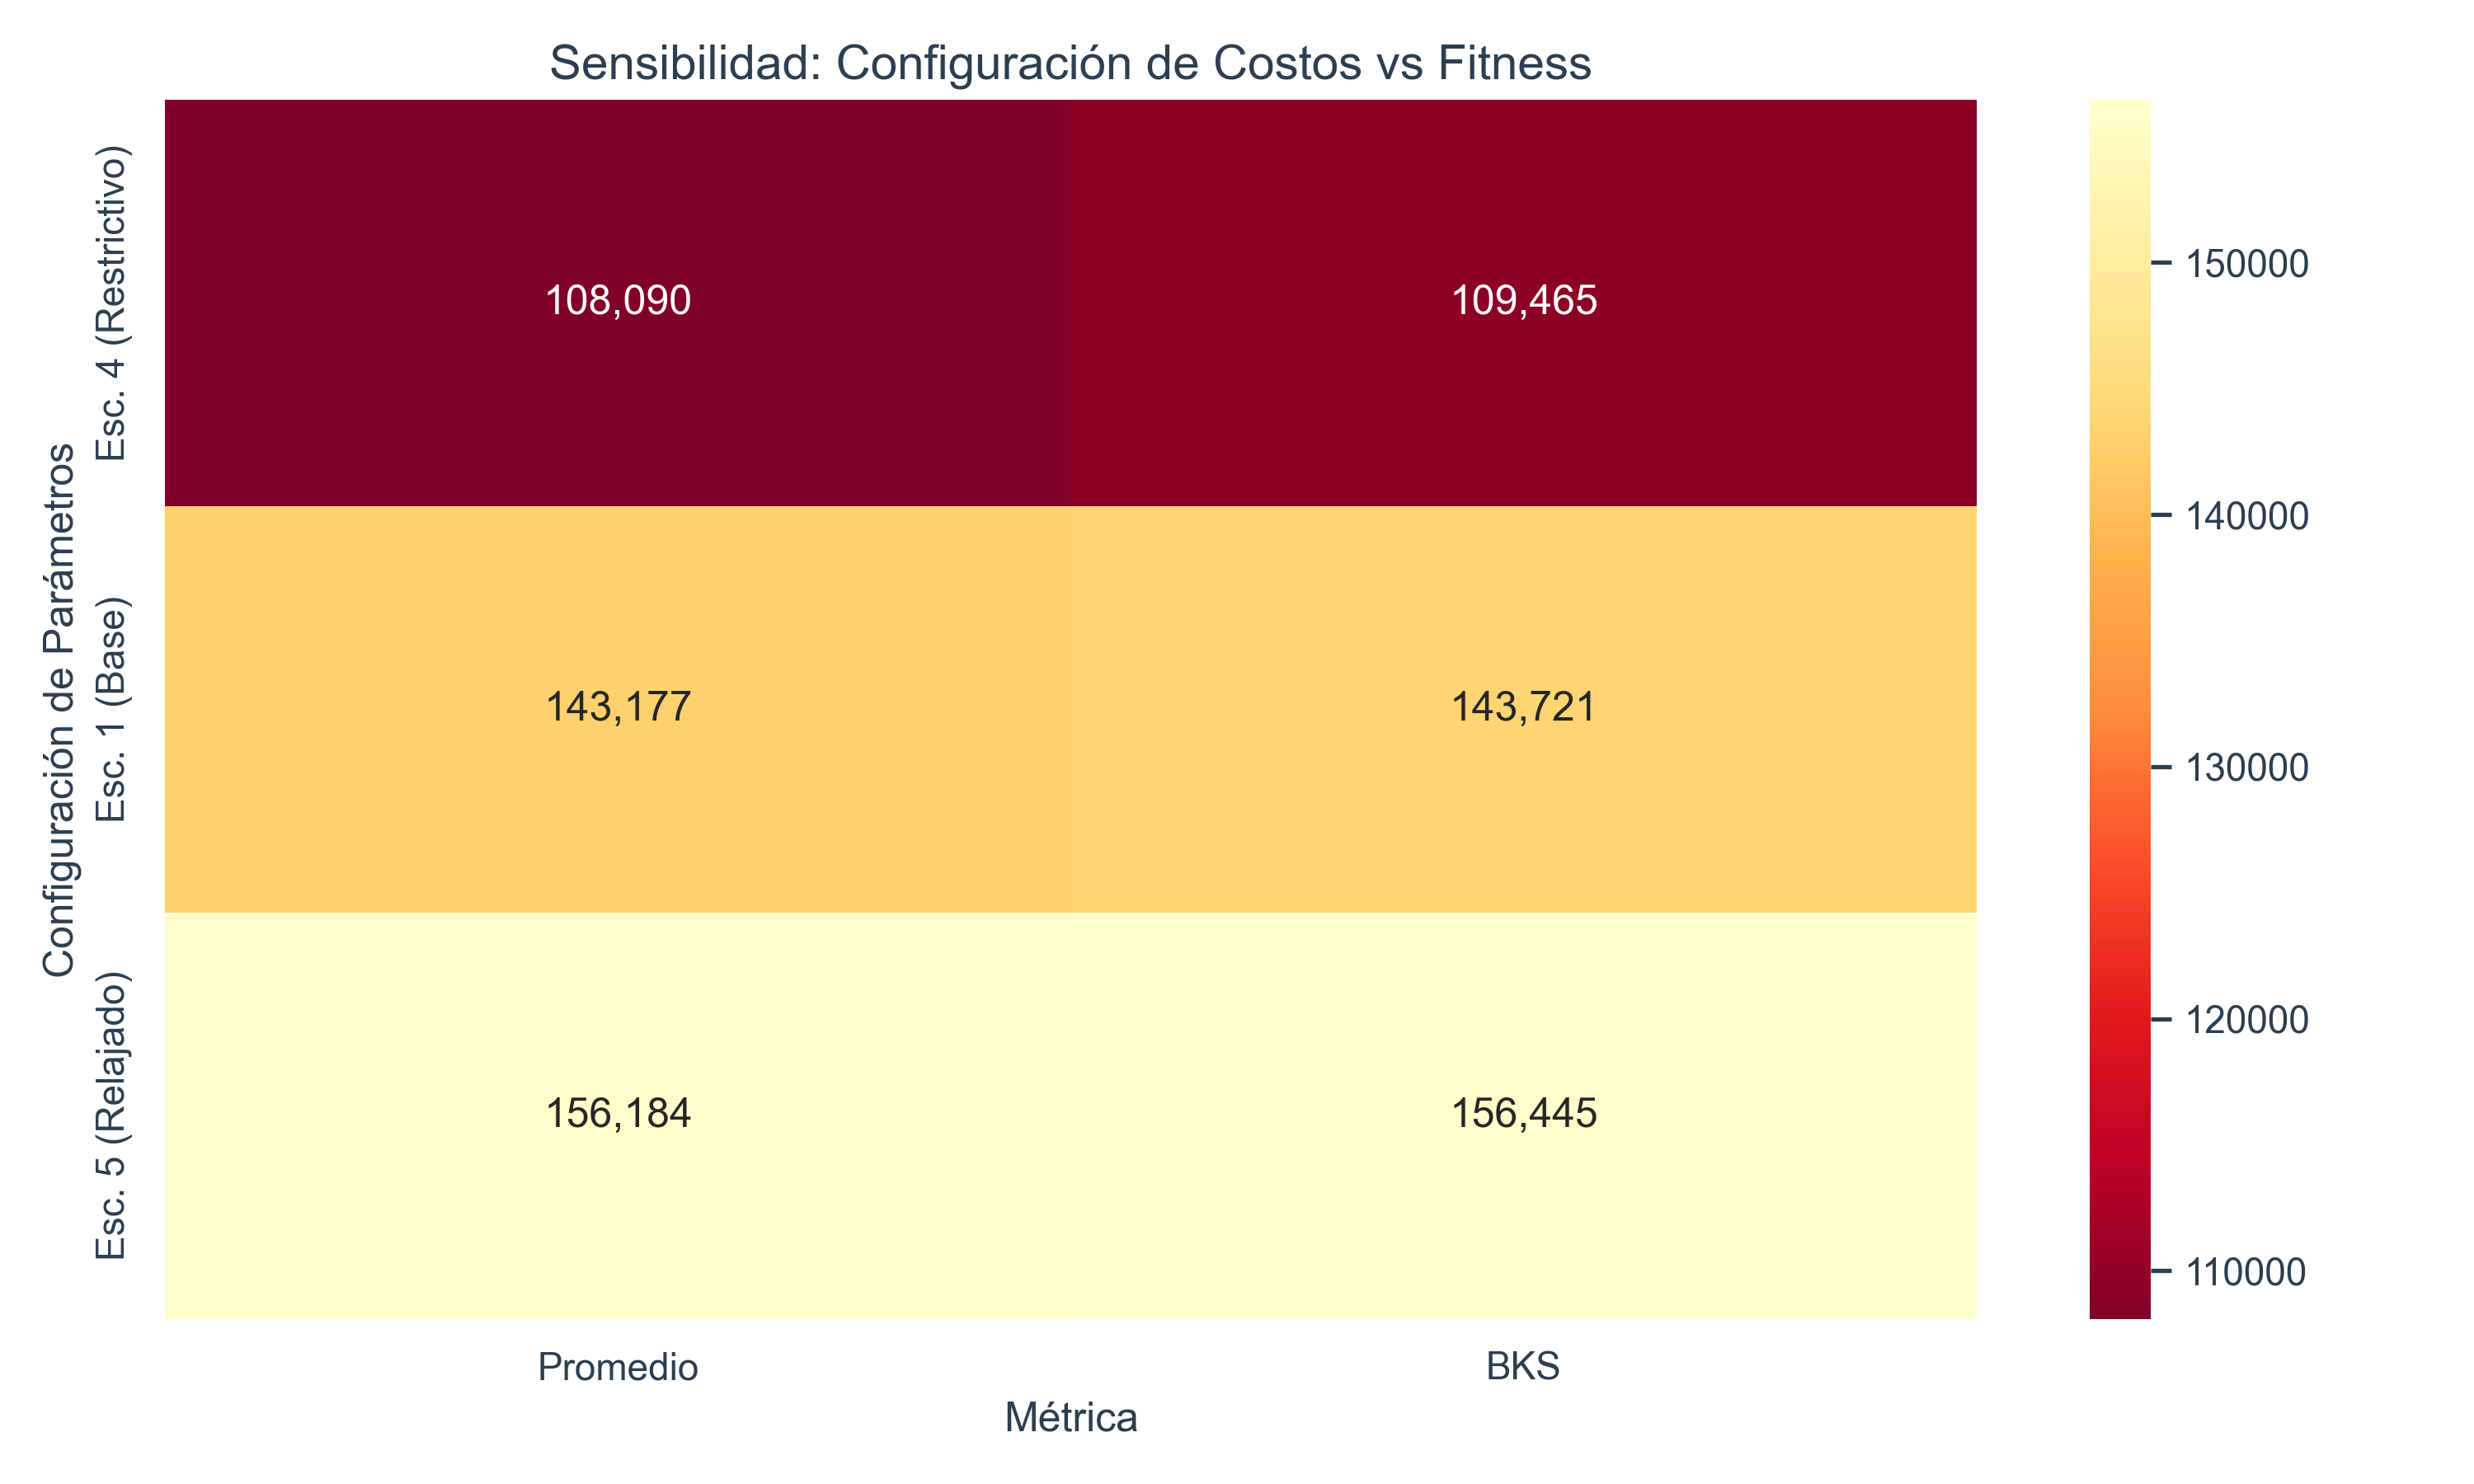
\includegraphics[width=0.85\textwidth]{../Figures/fig06_heatmap_params.png}
\caption{Heatmap de sensibilidad: configuración de costos vs fitness}
\label{fig:heatmap}
\end{figure}

\subsection{Escalabilidad}

\begin{figure}[H]
\centering
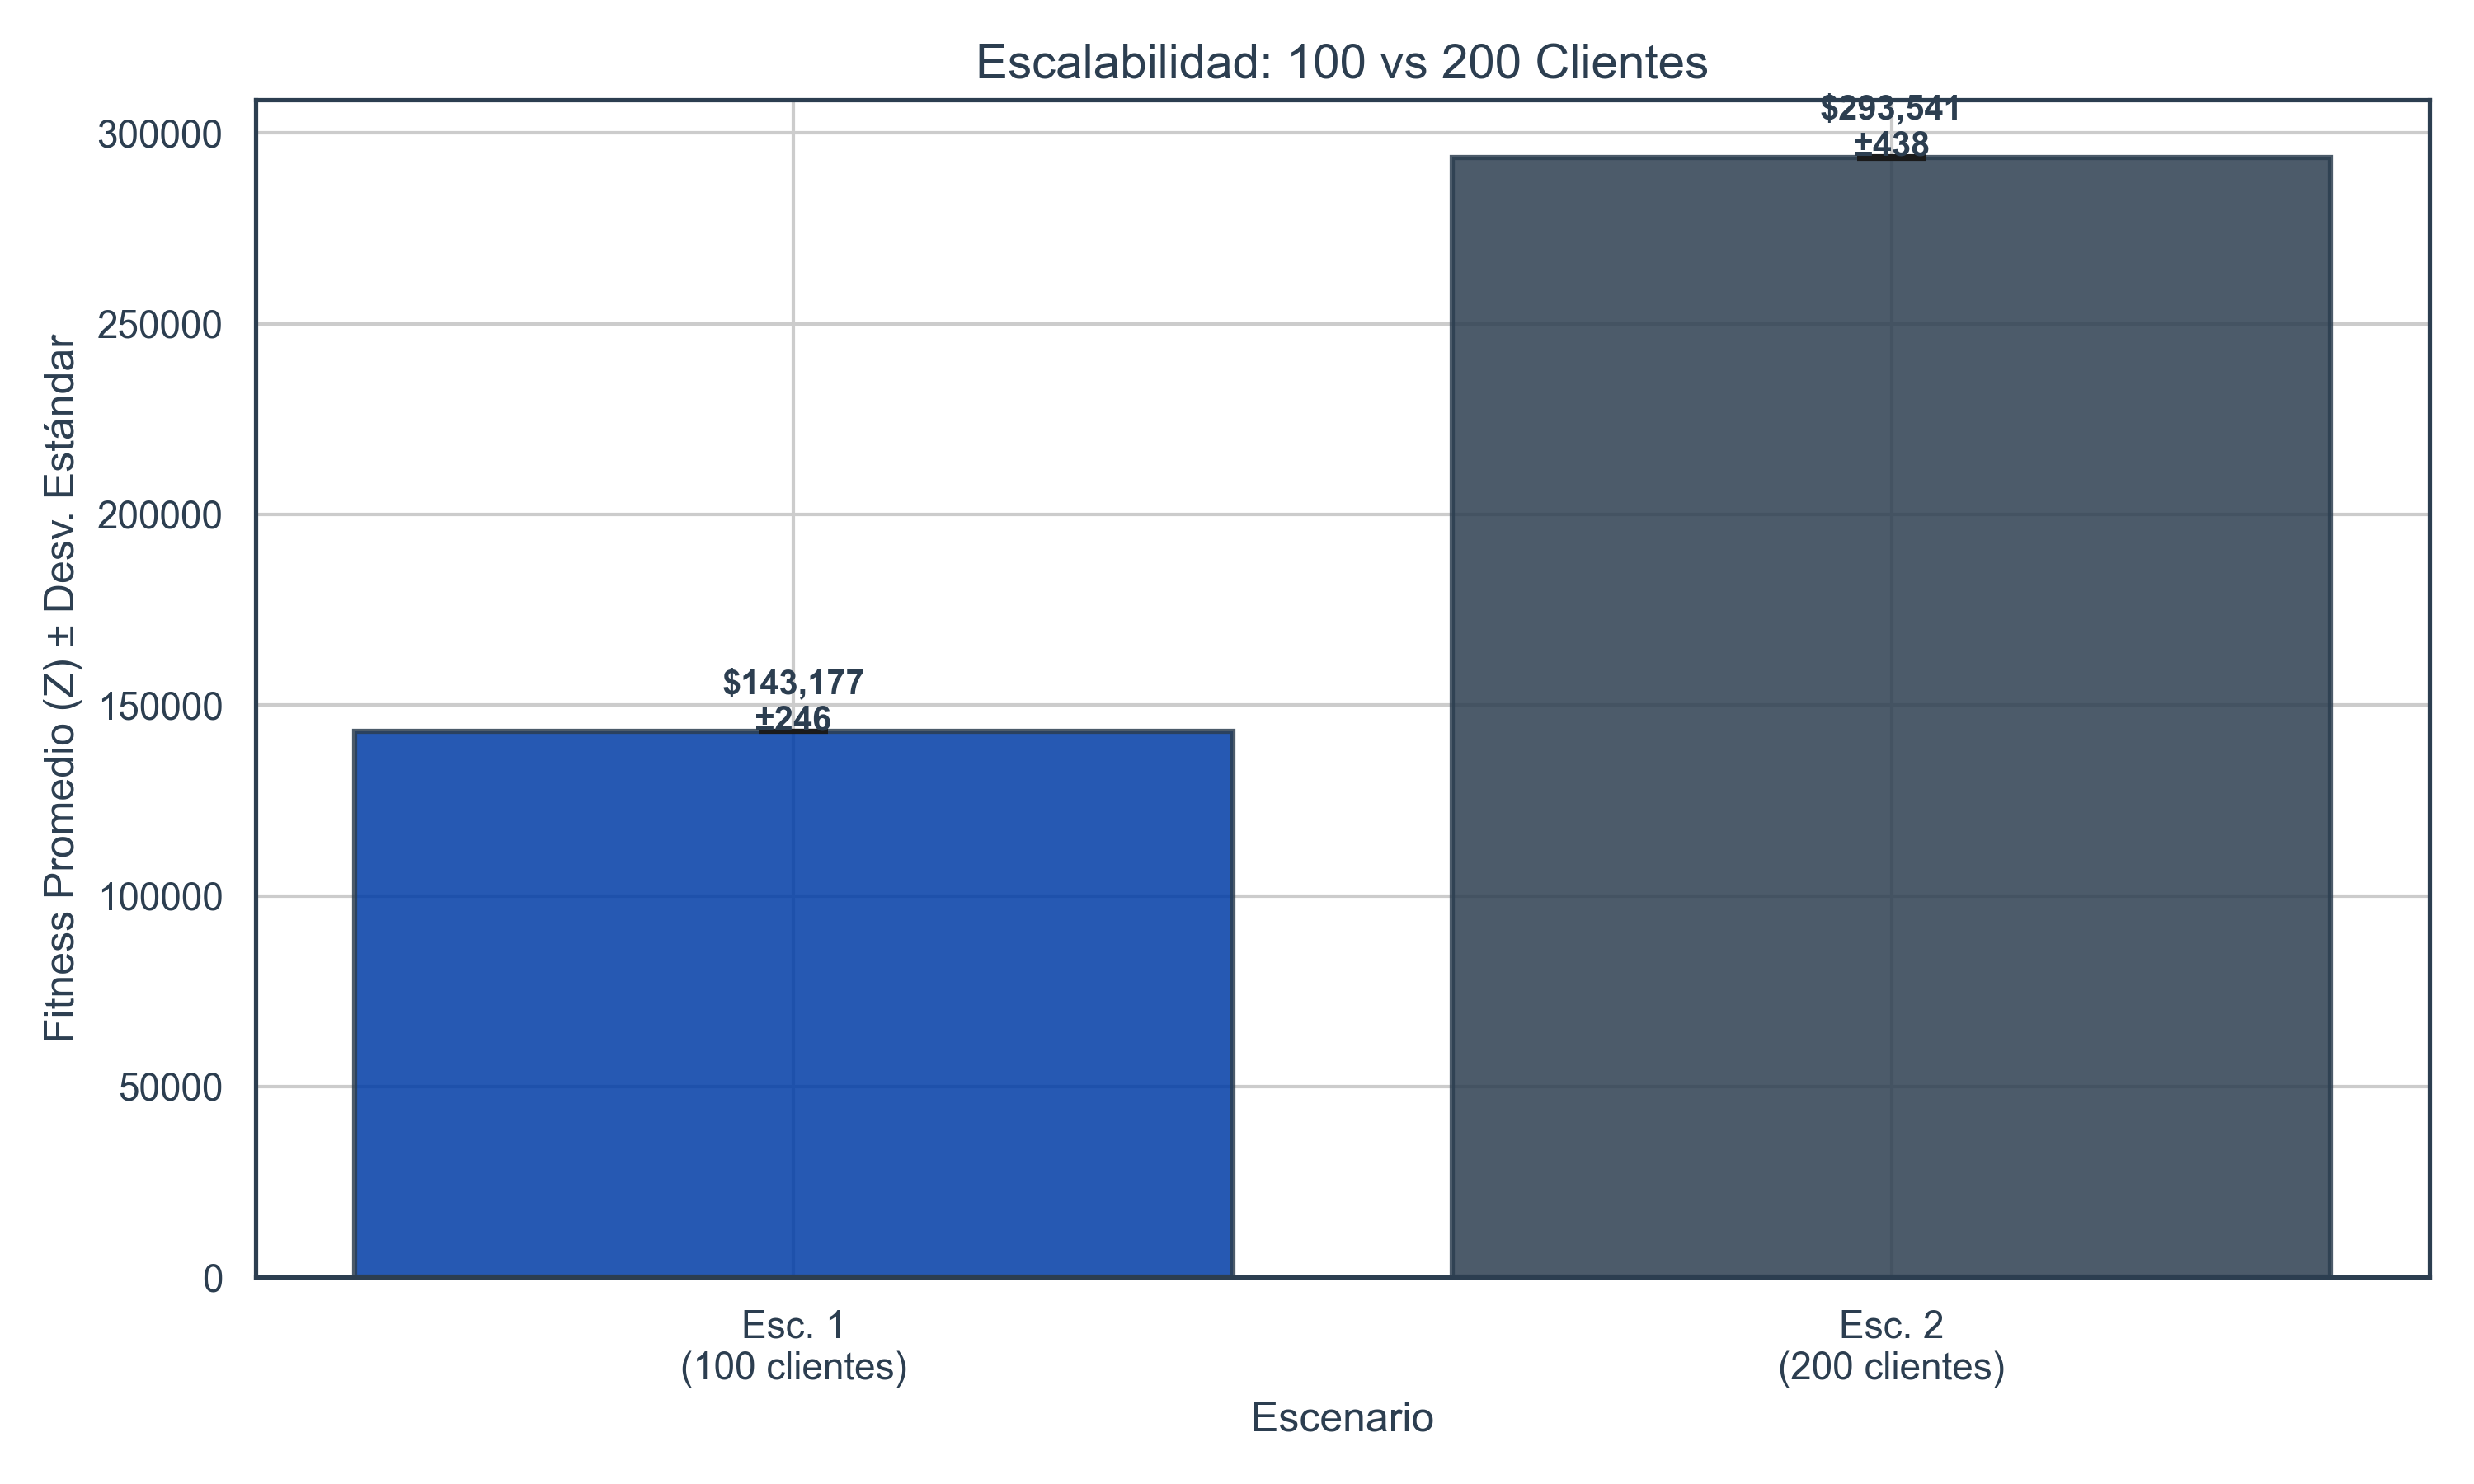
\includegraphics[width=0.85\textwidth]{../Figures/fig07_escalabilidad.png}
\caption{Comparación de escalabilidad: 100 vs 200 clientes}
\label{fig:scalability}
\end{figure}

% ============================================================
% 5. ANÁLISIS Y DISCUSIÓN
% ============================================================
\section{Análisis y Discusión}

\subsection{Degradación por Escalabilidad}
Al incrementar la dimensionalidad de 100 a 200 clientes (Escenarios 1 vs 2), se espera observar un incremento significativo en el Gap y una reducción en la Tasa de Éxito. Esto se debe a que el espacio de búsqueda crece factorialmente ($n!$ permutaciones), dificultando la convergencia del AG con los mismos hiperparámetros. El algoritmo requeriría mayor población y más generaciones para mantener la calidad de las soluciones.

\subsection{Impacto de las Penalizaciones}
La comparación entre los Escenarios 4 (penalizaciones altas) y 5 (penalizaciones relajadas) permite evaluar la sensibilidad del AG a la estructura de costos. Con penalizaciones altas, el algoritmo debe encontrar rutas más eficientes en términos de utilización de capacidad, lo que restringe el espacio de soluciones factibles de alta calidad. En contraste, con capacidades ampliadas y costos reducidos, el AG tiene mayor flexibilidad para consolidar rutas, resultando en soluciones de mayor ganancia neta.

\subsection{Variabilidad Económica}
El Escenario 3 (mercado premium) genera valores de fitness absolutos distintos debido a los mayores ingresos por unidad, pero el comportamiento estocástico del AG se mantiene similar. La menor demanda por cliente permite rutas con más clientes por vehículo, reduciendo el número de vehículos necesarios.

\subsection{Importancia de las 30 Ejecuciones}
Dado el carácter estocástico de los AG (inicialización aleatoria, selección por torneo, cruce y mutación probabilísticos), una sola ejecución no tiene validez estadística. Las 30 ejecuciones independientes permiten calcular medidas de tendencia central, dispersión y tasas de éxito que caracterizan fielmente el rendimiento del algoritmo.

% ============================================================
% 6. CONCLUSIONES
% ============================================================
\section{Conclusiones}

\begin{enumerate}
    \item \textbf{Comportamiento bajo estrés de escala:} El AG demuestra ser efectivo para instancias de tamaño medio (100 clientes), pero su rendimiento se degrada al escalar a 200 clientes sin ajustar hiperparámetros. Esto confirma la necesidad de estrategias adaptativas o hibridación con búsqueda local para problemas de mayor dimensionalidad.

    \item \textbf{Sensibilidad a parámetros de penalización:} La estructura de costos tiene un impacto directo en la calidad y estructura de las rutas generadas. Penalizaciones altas fuerzan soluciones más compactas pero de menor ganancia neta, mientras que costos relajados permiten mayor consolidación y rentabilidad.

    \item \textbf{Limitaciones y mejoras potenciales:} El AG implementado utiliza operadores básicos sin búsqueda local. Mejoras como la hibridación con 2-opt o 3-opt, el uso de algoritmos multi-objetivo como NSGA-II \cite{deb2002} para balancear costo y distancia simultáneamente, o esquemas de diversificación adaptativos, podrían mejorar significativamente el rendimiento.

    \item \textbf{Conexión con aplicaciones reales:} El VRP es análogo a problemas de asignación de recursos bajo restricciones presentes en múltiples industrias. En el sector bancario y fintech, la optimización de rutas para cajeros automáticos, la asignación de límites de crédito bajo restricciones de capital, y la planificación logística de efectivo son problemas estructuralmente similares donde las metaheurísticas evolutivas ofrecen soluciones prácticas.
\end{enumerate}

% ============================================================
% 7. REFERENCIAS
% ============================================================
\begin{thebibliography}{10}

\bibitem{porras2026}
R. G. Porras Alaniz, ``Programando un Algoritmo Genético desde Cero para el VRP,''
Universidad Autónoma de Ciudad Juárez (UACJ), 2026. [Online].
Available: AGfromscratch.html [Accessed: Mar. 8, 2026].

\bibitem{dantzig1959}
G. B. Dantzig and J. H. Ramser, ``The truck dispatching problem,''
\textit{Management Science}, vol. 6, no. 1, pp. 80--91, Oct. 1959.
doi: 10.1287/mnsc.6.1.80

\bibitem{davis1985}
L. Davis, ``Applying adaptive algorithms to epistatic domains,''
in \textit{Proc. Int. Joint Conf. Artificial Intelligence (IJCAI)}, 1985, pp. 162--164.

\bibitem{deb2002}
K. Deb, A. Pratap, S. Agarwal, and T. Meyarivan, ``A fast and elitist multiobjective
genetic algorithm: NSGA-II,'' \textit{IEEE Trans. Evol. Comput.}, vol. 6, no. 2,
pp. 182--197, Apr. 2002. doi: 10.1109/4235.996017

\bibitem{holland1975}
J. H. Holland, \textit{Adaptation in Natural and Artificial Systems}. Ann Arbor, MI:
University of Michigan Press, 1975.

\bibitem{toth2002}
P. Toth and D. Vigo, Eds., \textit{The Vehicle Routing Problem}. Philadelphia, PA:
SIAM Monographs on Discrete Mathematics and Applications, 2002.

\bibitem{vidal2020}
T. Vidal, G. Laporte, and P. Matl, ``A concise guide to existing and emerging
vehicle routing problem variants,'' \textit{European Journal of Operational Research},
vol. 286, no. 2, pp. 401--416, 2020. doi: 10.1016/j.ejor.2019.06.046

\bibitem{goldberg1989}
D. E. Goldberg, \textit{Genetic Algorithms in Search, Optimization, and Machine Learning}.
Reading, MA: Addison-Wesley, 1989.

\bibitem{michalewicz1996}
Z. Michalewicz, \textit{Genetic Algorithms + Data Structures = Evolution Programs}, 3rd ed.
Berlin, Germany: Springer, 1996.

\bibitem{oliveira2016}
F. B. de Oliveira, R. Enayatifar, H. J. Sadaei, F. G. Guimarães, and J.-Y. Potvin,
``A cooperative coevolutionary algorithm for the multi-depot vehicle routing problem,''
\textit{Expert Systems with Applications}, vol. 43, pp. 117--130, Feb. 2016.
doi: 10.1016/j.eswa.2015.08.030

\end{thebibliography}

% ============================================================
% 8. CONCLUSIÓN PERSONAL
% ============================================================
\section*{Conclusión Personal}

\begin{wrapfigure}{r}{0.25\textwidth}
    \centering
    % Uncomment when image is available:
    % \includegraphics[width=0.23\textwidth]{javiprofile.jpg}
    \vspace{-10pt}
\end{wrapfigure}

Esta actividad me permitió comprender a profundidad la mecánica interna de los Algoritmos Genéticos, desde la representación cromosómica hasta el diseño de operadores específicos para problemas de permutación como el VRP. La implementación desde cero, sin el uso de librerías de optimización, reforzó mi entendimiento de cada componente del proceso evolutivo.

El diseño experimental con múltiples escenarios me enseñó la importancia de evaluar metaheurísticas bajo condiciones variadas, ya que el rendimiento de un AG puede variar significativamente con cambios en la dimensionalidad del problema o en la estructura de costos. Las 30 ejecuciones independientes por escenario demostraron la naturaleza estocástica de estos algoritmos y la necesidad de métricas estadísticas robustas.

Desde mi experiencia profesional en el sector bancario y fintech, puedo identificar aplicaciones directas de estas técnicas en la optimización de rutas de cajeros automáticos, la asignación dinámica de recursos, y la planificación logística — problemas que comparten la misma estructura combinatoria que el VRP.

\vspace{0.5cm}
\noindent\textbf{Javier Augusto Rebull Saucedo} \\
Matrícula: 263483 \\
MIAAD — UACJ

\end{document}
